\documentclass{article}
\usepackage{graphicx} % Required for inserting images
\usepackage{enumitem}
\usepackage{amsmath}
\usepackage{array}
\usepackage{amssymb}
\usepackage{tikz}
\usepackage{titling}
\newcommand{\subtitle}[1]{%
  \posttitle{%
    \par\end{center}
    \begin{center}\large#1\end{center}
    \vskip0.5em}%
}
\makeatletter
\newcommand\setItemnumber[1]{\setcounter{enum\romannumeral\@enumdepth}{\numexpr#1-1\relax}}
\makeatother
\title{MATH 304: Homework 3}
\subtitle{Case Western Reserve University}
\author{Rohan Rajappan \\rohan@case.edu}
\date{February 14, 2024}
\begin{document}

\maketitle

\section{3.1}
 \paragraph{Problems: 4ab, 7cd, 12, 17b, 20, 22a, 28}
 \begin{enumerate}
     \setItemnumber{4}
     \item Let $Q(n)$ be the predicate $n^2 \leq 30$
     \begin{enumerate}
         \item $Q(2) = 4\leq 30$ is a true statement. 

         $Q(-2) = 4\leq 30$ is a true statement.

         $Q(7) = 49\leq 30$ is a false statement.

         $Q(-7) = 49\leq 30$ is a false statement.
         \item $\{n \in \mathbb{Z} \mid Q(n)\} = \{n \in \mathbb{Z} \mid -5 \leq n \leq 5\} = \{-5, -4, -3, -2, -1, 0, 1, 2, 3, 4, 5\}$
     \end{enumerate}
     \setItemnumber{7}
     \item Find the truth set of each predicate
     \begin{enumerate}
         \setItemnumber{3}
         \item $R(x) = 1\leq x^2\leq4.$ The truth set on the domain $\mathbb{R}$ is $\{x\in\mathbb{R}\mid -2 \leq x \leq -1 \lor 1 \leq x \leq 2\} $
         \item $R(x) = 1\leq x^2\leq4.$ The truth set on the domain $\mathbb{Z}$ is $\{x\in\mathbb{Z}\mid -2 \leq x \leq -1 \lor 1 \leq x \leq 2\} $
     \end{enumerate}
     \setItemnumber{12}
     \item $\forall\:x, y \in \mathbb{R}:  \sqrt{x+y} = \sqrt{x}+\sqrt{y}$ can be disproved in the case that $x,y = 2$ as $\sqrt{2+2} = \sqrt{4} = 2$, yet
     $\sqrt{2} + \sqrt{2} = 2\sqrt{2}$ and $2 \neq 2\sqrt{2}$.
     \setItemnumber{17}
     \item 
     \begin{enumerate}
         \setItemnumber{2}
         \item There exists a rational number x, such that x is a real number.
     \end{enumerate}
     \setItemnumber{20}
     \item (1) Given any real number, if the number is positive, then the square root is also positive. (2) The square root of any positive real number is also positive.
     \setItemnumber{22}
     \item 
     \begin{enumerate}
         \item $\forall x$, if $x$ is a Java program, then $x$ has at least 5 lines.
     \end{enumerate}
     \setItemnumber{28}
     \item Let the domain of $x$ be the set $D$ of objects discussed in mathematics courses, and let $Real(x)$ be ``$x$ is a real number,” $Pos(x)$ be ``$x$ is a positive real number,” $Neg(x)$ be ``$x$ is a negative real number,” and $Int(x)$ be ``$x$ is an integer.”
     \begin{enumerate}
         \item The statement $Pos(0)$ states that 0 is a positive real number. This is a false statement as 0 is not greater than 0. Thus, 0 cannot be a positive real number.
        \item The statement $\forall x, Real(x) \land Neg(x) \rightarrow Pos(-x)$ means that if x is a negative real number, the opposite of x will be positive. This is a true statement. The opposite of any negative number will be positive. Thus, for any real negative number, the opposite must be positive.
        \item The statement $\forall x, Int(x) \rightarrow Real(x)$ means that if x is an integer, x must be real number. This is a true statement. All integers are whole numbers, thus this statement is true.
        \item $\exists x, $ such that $Real(x) \land \sim Int(x)$ means that there is an x such that x is a real number but not an integer. This is a true statement. One example of this is 0.2 as it is a real number, yet it is not an integer.
     \end{enumerate}
 \end{enumerate}
  
\section{3.2}
\paragraph{Problems: 1, 5, 12, 17, 29, 48}
\begin{enumerate}
    \item Options a (``There is a discrete mathematics student who is nonathletic.") and e (``Some discrete mathematics students are nonathletic.") are proper negations of the statement.
    \setItemnumber{5}
    \item Write a negation for each of the following statements
    \begin{enumerate}
        \item ``Every valid argument has a true conclusion." $\rightarrow$ There exists a valid argument that does not have a true conclusion.
        \item ``All real numbers are positive, negative, or zero" $\rightarrow$ There exists a real number that is neither positive, negative, nor zero.
    \end{enumerate}
    \setItemnumber{12}
    \item Statement: ``The product of any irrational number and any rational number is irrational."

    Proposed Negation: ``The product of any irrational number and any rational number is rational."

    This is not a proper negation. In this case, they only negated the conclusion of the statement. Additionally, they changed ``irrational" to ``rational". In this case, it is fine as numbers can only be rational or irrational. To be safe, however, it could have been ``..any rational number is not irrational". The premise should not use the word ``any" as it implies this is a universal statement. Instead, it should state the existence of at least a singular case.
    \setItemnumber{17}
    \item $\exists$ an integer $d$ such that $6/d$ is an integer and $d\neq 3$.
    \setItemnumber{29}
    \item Statement from problem 19: ``$\forall n\in\mathbb{Z}$, if $n$ is prime, then $n$ is odd or $n=2$"

    Inverse: $\forall n\in\mathbb{Z}$, if $n$ is not prime, then $n$ is not odd and $n\neq2$ This is false. A non-prime number can be odd. For example, 25 is not prime, yet 25 is odd. Thus this statement is proven false by counterexample.

    Converse: $\forall n\in\mathbb{Z}$, if $n$ is odd or $n=2$, then $n$ is prime. This is false. A number can be odd but not prime. For example, 15 is odd, yet 15 is $3*5$ and is therefore not prime. Thus, this statement is proven false by counterexample.

    Contrapositive: $\forall n\in\mathbb{Z}$, if $n$ is not odd or $n\neq2$, then $n$ is not prime. This is a true statement.
    \setItemnumber{48}
    \item ``Being a polynomial is not a sufficient condition for a function to have a real root." means that there exists a polynomial such that there is not a real root. In other words, $\exists$ an equation $x$, such that $x$ is a polynomial and $x$ does not have any real roots.
\end{enumerate}
\section{3.3}
\paragraph{Problems: 2, 10ab, 19, 23}
\begin{enumerate}
    \setItemnumber{2}
    \item Let $G(x, y)$ be $x^2>y$ Indicate which of the following statements are true and which are false.
    \begin{enumerate}
        \item $G(2,3)$ is true as $2^2 =4$ thus $4>3$, which is a true statement.
        \item $G(1,1)$ is not true as $1^2 = 1$ thus making the statement is $1>1$, which is not true.
        \item $G(\frac{1}{2},\frac{1}{2})$ is not true as $(\frac{1}{2})^2=\frac{1}{4}$ and $\frac{1}{4}>\frac{1}{2}$ is not a true statement.
        \item $G(-2,2)$ is a true statement as $(-2)^2=4$ and $4>2$ is a true statement.
    \end{enumerate}
    \setItemnumber{10}
    \item This exercise refers to Example 3.3.3. Determine whether each of the following statements is true or false.
    \begin{enumerate}
        \item $\forall$ student $S$, $\exists$ a dessert $D$ such that $S$ chose $D$. This is true as each student chose at least one dessert. Thus, for all students, there exists a dessert that was chosen by the student.
        \item $\forall$ student $S$, $\exists$ a salad $T$ such that $S$ chose $T$. This is not true. What this means is that for all students, there exists a salad such that the student chose the salad. This is untrue because Yuen did not choose a salad.
    \end{enumerate}
    \setItemnumber{19}
    \item $\exists x\in\mathbb{R}$ such that for every real number $y$, $x+y=0$.
    \begin{enumerate}
        \item This means that there exists a real number such that when it is added to every real number, it is 0 in every case.
        \item Negation: $\forall x \in\mathbb{R}$,  such that for every real number $y$, $x+y\neq0$
    \end{enumerate}
    \setItemnumber{23}
    \item 
    \begin{enumerate}
        \item $\forall$ nonzero number $r$, $\exists$ a real number $s$, such that $rs = 1$. 
        
        This means that for every real number, there exists a real number of which the product of the two numbers will equal 1. This statement is true. For any real number, you can multiply the number by its reciprocal, and the product will be 1.
        \item $\exists$ a real number r such that $\forall$ nonzero real numbers s, $rs=1$.

        This means that there must exist a nonzero real number such that for all nonzero real numbers, the product of the two numbers is 1. This is not a true statement. This statement states that there is one nonzero real number which equates to 1 when multiplied by any other nonzero real number. There is not a single number that does this.
    \end{enumerate}
\end{enumerate}

\section{3.4}
\paragraph{Problems: 2, 14, 22, 24}
\begin{enumerate}
    \setItemnumber{2}
    \item If an integer $n$ equals $2*k$ and $k$ is an integer, then $n$ is even.

    0 is an integer.

    $2*0 = 0$.

    Therefore, due to universal instantiation, 0 must be even. Since 0 is an integer, $2*0=0$, and any integer multiplied by 2 is even, 0 must be even.
    \setItemnumber{14}
    \item ``If compilation of a computer program produces error messages, then the program is not correct." 
    
    ``Compilation of this program does not produce error messages."

    ``$\therefore$ This program is correct."

    This is an invalid argument. This is an inverse error. Although the computer program does not produce an error message, that does not imply that the program is correct.
    \setItemnumber{22}
    \item 
    ``All discrete mathematics students can tell a valid argument from an invalid one."
    
    ``All thoughtful people can tell a valid argument from an invalid one." 
    
    ``$\therefore$ All discrete mathematics students are thoughtful."

    This is an invalid argument. All discrete mathematics students and all thoughtful people are in the group of being able to tell a valid argument from an invalid one. This premise, however, does not imply that all discrete mathematics students fall in the category of thoughtful. They can share a parent category but not be the same.

    
    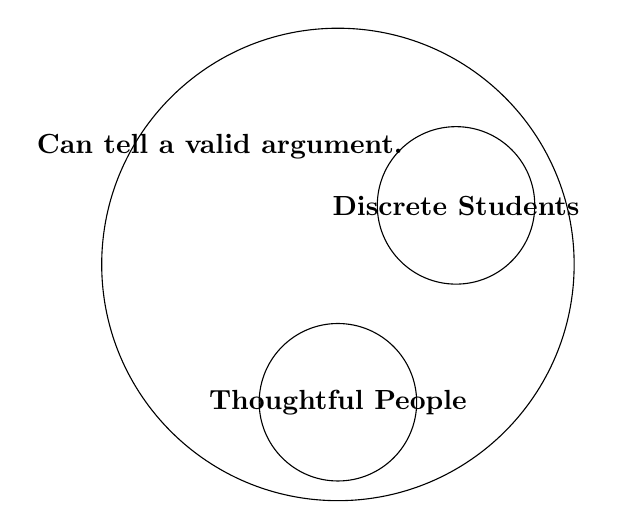
\begin{tikzpicture}
	\begin{scope} [fill opacity = 1]
    \draw[draw = black] (0,0) circle (3);
    \draw[draw = black] (1.5,.75) circle (1);
    \draw[draw = black] (0,-1.75) circle (1);
%% We can use the node command to label points. If you put your cursor on "LARGE" or "textbf" a box will drop down with size and text style options.
    \node at (-1.5,1.5) {\textbf{Can tell a valid argument.}};
    \node at (1.5,.75) {\textbf{Discrete Students}};
    \node at (0,-1.75) {\textbf{Thoughtful People}};
    \end{scope}
\end{tikzpicture}
\setItemnumber{24}
\item ``No vegetarians eat meat." 

``All vegans are vegetarian." 

``$\therefore$ No vegans eat meat."

This is a valid argument. As seen in the diagram below. No vegetarians eat meat, thus the circles are separate. Since all vegans are categorized under vegetarians, that means that no vegan can eat meat. Thus, this argument is valid.

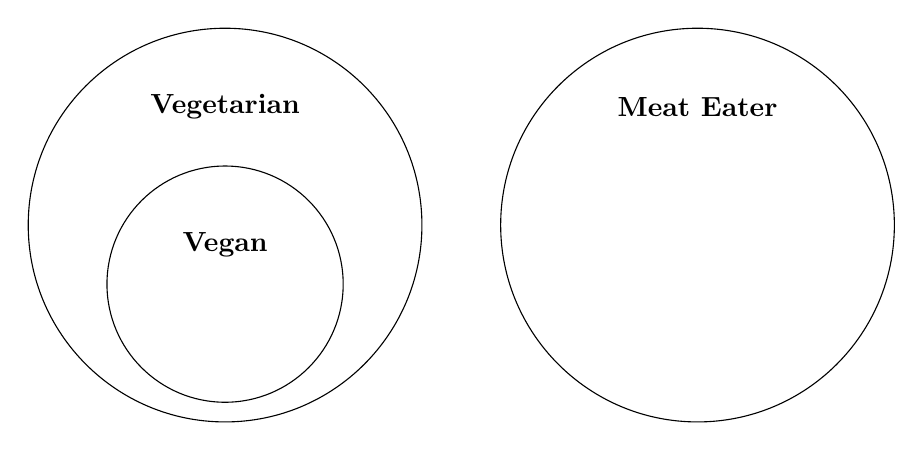
\begin{tikzpicture}
	\begin{scope} [fill opacity = 1]
    \draw[draw = black] (-3,-1) circle (2.5);
    \draw[draw = black] (3,-1) circle (2.5);
    \draw[draw = black] (-3,-1.75) circle (1.5);
%% We can use the node command to label points. If you put your cursor on "LARGE" or "textbf" a box will drop down with size and text style options.
    \node at (-3, .5) {\textbf{Vegetarian}};
    \node at (-3,-1.25) {\textbf{Vegan}};
    \node at (3,.5) {\textbf{Meat Eater}};
    \end{scope}
\end{tikzpicture}
    
\end{enumerate}
\end{document}
